\section{Développement}
Après avoir testé tout le panel des IDEs compatibles JavaEE, nous nous sommes arrêté sur IntelliJ-Idea Ultimate a l'aide de licences étudiantes gratuites.
L'outil permet de créer des projets Java web, possède des plugins TomCat, Maven, Git. Il fonctionne sur toutes nos machines.
Une fois l'environnement de développement choisi, nous commençons d'abord par essayer de concevoir le site 'from scratch', sans aucun framework, avec les Servlets et JSP comme seules fondations.
Cette première esquisse nous permet de de commencer le développement du client et ainsi finaliser la conception de la base de donnée grâce des mock-ups simples.
Nous réalisons ensuite l'ampleur de la tâche qu'il nous reste a abattre et choississons de nous tourner vers Spring et Hibernate après une très brêve étude des non-alternatives autorisées par le sujet.

\subsection{Schéma de l'application}

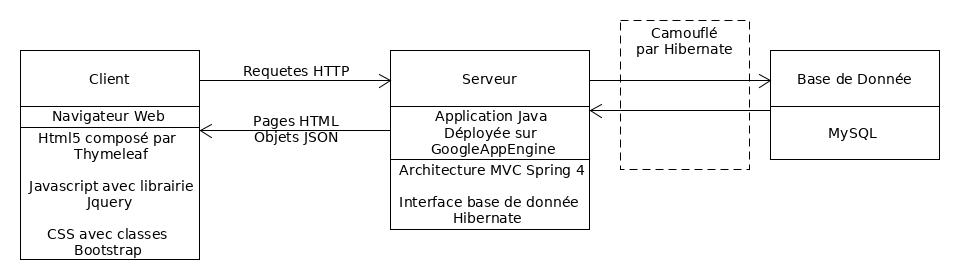
\includegraphics[width=\linewidth]{ApplicationSchema.jpg}

\subsection{Technologies}

\subsubsection{Spring}
Nous avons en particulier profité de Spring Security, qui propose des mesures de securité pour l'application appliquées de manière automatique: celles ci incluent la protection contre les attaques CSRF (en toujours ajoutant un champ contenant un token aux forms) et une gestion securisée des utilisateurs (système d'authentification, roles des comptes et cryptation secure des mots de passe à l'aide d'un hash sha-256 et d'un salt).

\subsubsection{Hibernate}
En ce qui concerne les données persitantes, nous avons utilisé l'ORM Hibernate en conjoction avec JPA. Le premier nous garanti un système automatique de mapping entre les objets et la BDD en écriture et en lecture; le deuxieme nous permet d'ecrire les configurations de persistance des entités grace a des annotations Java plutot que des fichiers configuration XML. Ce qui est beaucoup plus pratique.
Nous avons reussi à beaucoup modulariser le code en suivant l'architecture MVC plus quelques services et annotation (surtout pour ce qui concerne la validation des entités et l'injection d'entités dans les controleurs).

\subsubsection{Thymeleaf}
Nous profitons de ce moteur de templating pour générer dynamiquement les pages HTML en fonctions des valeurs des attributs mis à jour dans les Controller.

\subsubsection{MySQL}
Nous avons choisit MySQL a cause de multiples raisons. Il est gratuit, puisant, efficace et compatible avec Hibernate.
Mais ce ne sont pas seulement ces avantages qui ont motivé notre choix.

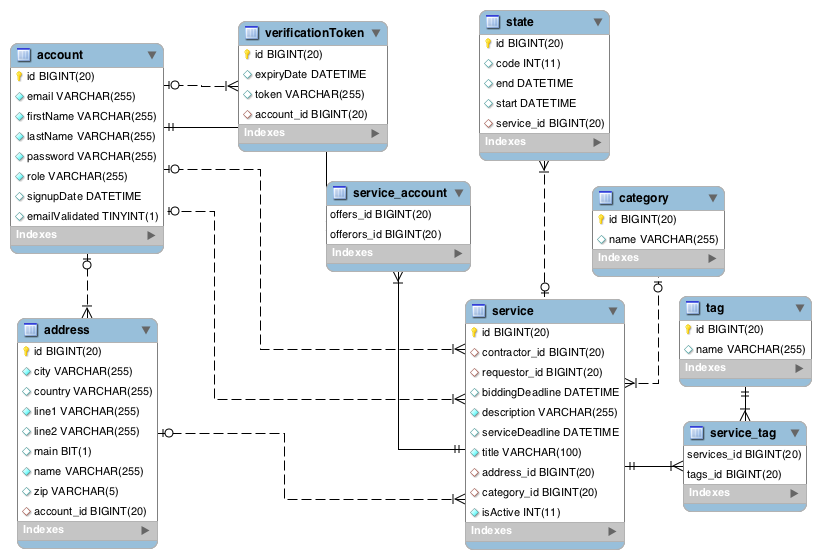
\includegraphics[width=\linewidth]{schemaBDD.png}
\begin{center}
\textit{Schéma de notre BDD.}
\end{center}

Le schéma de bases des données explique tout. Il n’est pas énormément complexe mais les relations entre les tables sont nombreuses. Ca veut dire qu'une base de données orientée documents n’est pas ni optimale ni facile à utiliser. Par exemple, l'entité Service a des liaison avec avec les autres tables. Dans une base de données orientée documents, les résultats des "query" pourraient être très grand et peu flexibles. De plus, certaines données pourraientt être dupliquées inutilement, comme « Category » et « Tag ».
\newline
Pour toutes ces raisons nous avons choisit MySQL.

\subsubsection{jQuery et Bootstrap}
Pour la partie client de l'application, nous avons choisit d'utiliser les frameworks jQuery et Bootstrap. Le premier nous permet de simplifier l'écriture de code java-script tout en s'assurant la compatibilité avec les differents navigateurs. L'autre nous donne accès à un ensemble de classes CSS qui rendent notre interface "responsive", en s'adaptant à toute taille d'écran (des smartphone aux plus grands écrans des ordinateurs de bureau).
